\section{Utilisation du logiciel}

Les deux objectifs présentés en \ref{obj} étaient à l'origine plus vagues. Nous avions le choix entre pousser l'analyse très loin et ne pas faire une interface graphique très évoluée, ou trouver un juste milieu. Ambitieux, nous souhaitions pousser l'analyse loin et réaliser une interface graphique évoluée.

\subsection{Fonctionnement global}
A partir de fichiers de données recensant la topologie d'internet et sa structure. Nous devons, entre autre, construire un graphe et permettre son affichage dans une fenêtre en Qt.

Nous venons de voir que la base de l'application est \textit{Boost} et que nous avons adopté le pattern MVC afin de développer de manière plus sereine. La coeur de ce système est la communication entre le modèle et la vue, en d'autres termes : le contrôleur. Voici la liste de ses fonctionnalités :
\begin{itemize}
 \item lancer la lecture des fichiers de données afin de construire le graphe,
\item obtenir le nombre d'AS, de liens, et d'autres informations globales sur le graphe,
\item de récupérer le graphe sans les stubs,
\item de récupérer l'adjacence d'un AS,
\item de récupérer les informations concernant un AS (centrality, numéro),
\item de ne récupérer qu'une partie du graphe en fonction de la centralité des sommets,
\item de calculer les coordonnées que les sommets doivent avoir sur l'interface graphique.
\end{itemize}

L'ensemble de ses fonctionnalités se retrouve dans l'interface graphique, qui sera présentée ci-dessous.

%ATTENTION : \'ebauche pour cette partie.
\subsection{Description du programme}

Le programme tel que le voit l'utilisateur est une fen\^etre graphique avec un menu en haut, une zone d'affichage au centre, et une zone de notification en bas.

\begin{figure}[H]
\centering
 \fbox
 {
 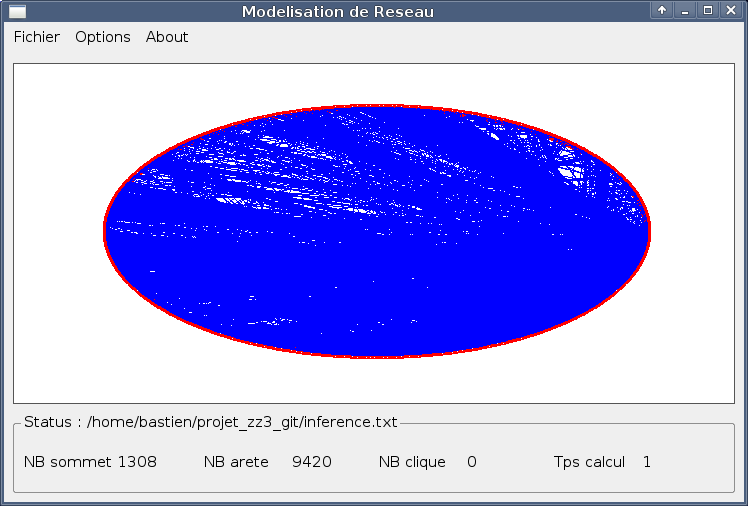
\includegraphics[width=16cm]{./schema/capture_ecran_programme.png}
 }
  \caption{\label{ecran_principal}Ecran principal du programme}
\end{figure}


Le menu comporte trois types d'entr\'ees :
\begin{description}
 \item[Fichier] permet l'ouverture des fichiers de donn\'ees \`a lire ou la fermeture du programme,
 \item[Options] permet les interactions avec le graphe telles que l'effacement de la zone d'affichage ou encore les recherche d'informations sur un AS,
 \item[About] permet l'affichage d'informations sur le programme.
\end{description}

\par
De nombreuses options sont disponibles pour l'utilisateur, et selon celles qu'il choisira d'utiliser, il en d\'ebloquera d'autres. Ces options permettent de jouer sur l'affichage du graphe et d'obtenir des informations sur les AS. Il y a :
\begin{itemize}
 \item R\'ecup\'eration d'informations sur un AS,
 \item Calcul du nombre de clique dans le graphe,
 \item Chargement d'un fichier de triplets pour \'eliminer les stubs du graphe,
 \item Zoomer sur le proche voisinage d'un AS,
 \item Revenir au graphe de base,
 \item Calculer la centralit\'e des sommets,
 \item Afficher seulement les sommets avec un poids sup\'erieur \`a une certaine valeur,
 \item Afficher seulement les sommets avec un poids inf\'erieur \`a une certaine valeur
 \item Afficher seulement les sommets avec un num\'ero d'AS sup\'erieur \`a une certaine valeur,
 \item Afficher seulement les sommets avec un num\'ero d'AS inf\'erieur \`a une certaine valeur
 \item effacer le graphe pour commencer une nouvelle \'etude.
\end{itemize}

Ces fonctions sont d\'ebloqu\'ees comme suit :

\begin{figure}[H]
\centering
 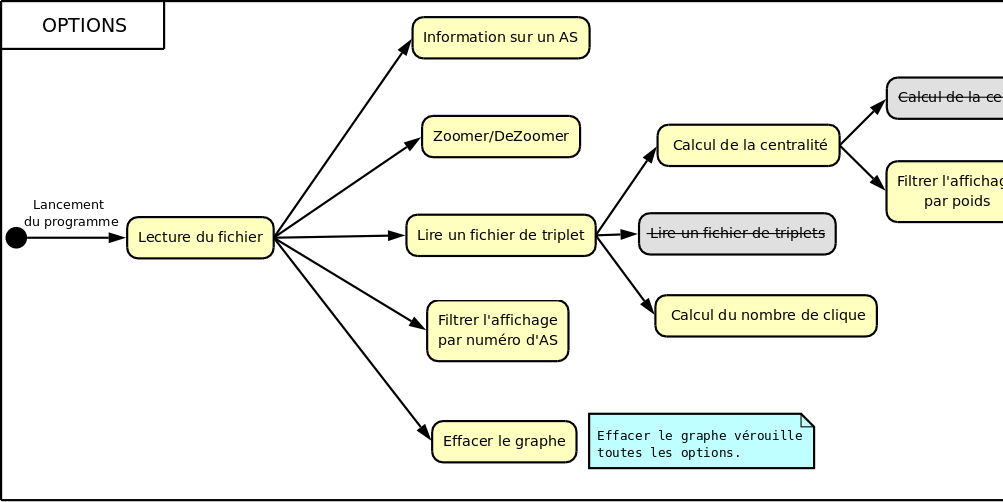
\includegraphics[width=0.8\textwidth]{./schema/seqMenu.png}
  \caption{\label{seq_option}S\'equence des d\'eve\'erouillage d'options}
\end{figure}


\subsection{L'exp\'erience utilisateur}
\par
Lors du lancement du programme, l'utilisateur se retrouve devant un fen\^etre o\`u la zone d'affichage est vide et les compteurs de la zone de notification sontt tous \`a z\'ero comme c'est le cas sur la figure \ref{ecran_principal}.
\par
\`A ce stade l\`a, l'utilisation des options ne lui est d'aucune utilit\'e car elles sont toutes bloqu\'ees en attendant qu'il charge un fichier. Il peut aller dans le menu \textit{About} pour avoir des informations sur le programme, comme montrt\'e figure \ref{ecran_about}.

\begin{figure}[H]
\centering
 \fbox
 {
 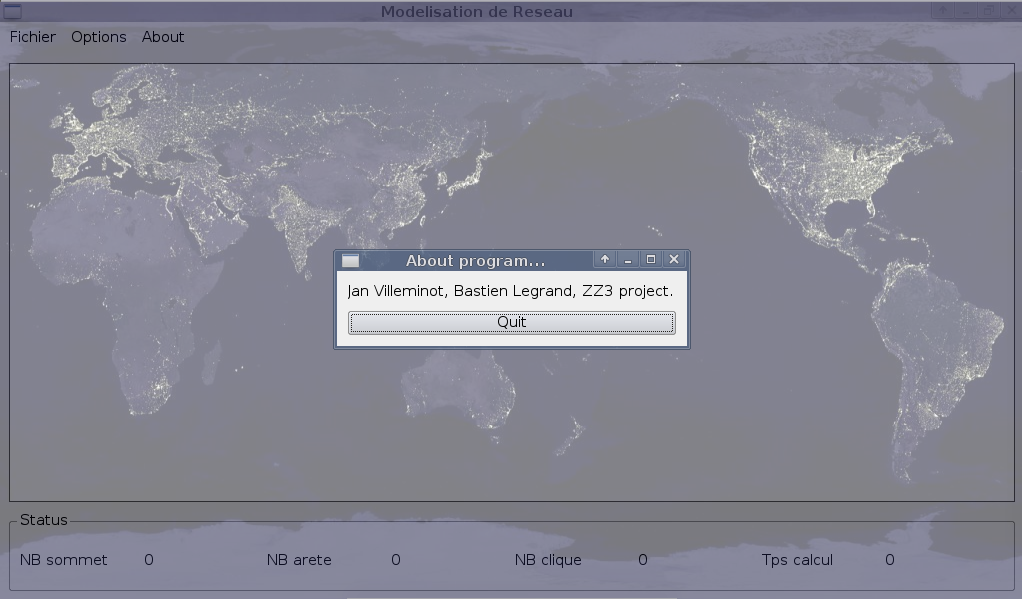
\includegraphics[width=16cm]{./schema/capture_ecran_about.png}
 }
  \caption{\label{ecran_about}Informations sur le programme}
\end{figure}

\par
Il peut aussi d\'ecider d'aller explorer le menu \textit{Fichier}, ce qui lui laissera le choix entre ouvrir un fichier de donn\'ees pour construire un graphe ou quitter le programme. Ce menu est illustr\'e figure \ref{ecran_fichier}.

\begin{figure}[H]
\centering
 \fbox
 {
 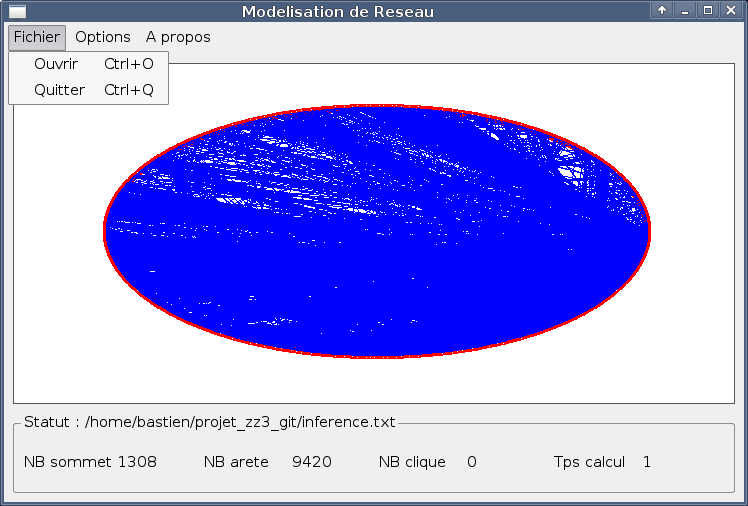
\includegraphics[width=16cm]{./schema/capture_ecran_fichier.png}
 }
  \caption{\label{ecran_fichier}Menu fichier}
\end{figure}

S'il choisit d'ouvrir un fichier de donn\'ees, une nouvelle fen\^etre de navigation s'ouvre et lui demande de choisir son fichier.

L'utilisateur choisit un fichier de donn\'ees \`a ouvrir et le logiciel se charge d'afficher le graphe correspondant en organisant les sommets sur un polyg\^one r\'egulier \`a n c\^ot\'es.
La barre de status est mise \`a jour avec des informations telles que le nombre de sommets, le nombre d'ar\^etes ou le temps de calcul. Il obtient ainsi un \'ecran comme on peut en voir un figure \ref{ecran_graph}

\begin{figure}[H]
\centering
 \fbox
 {
 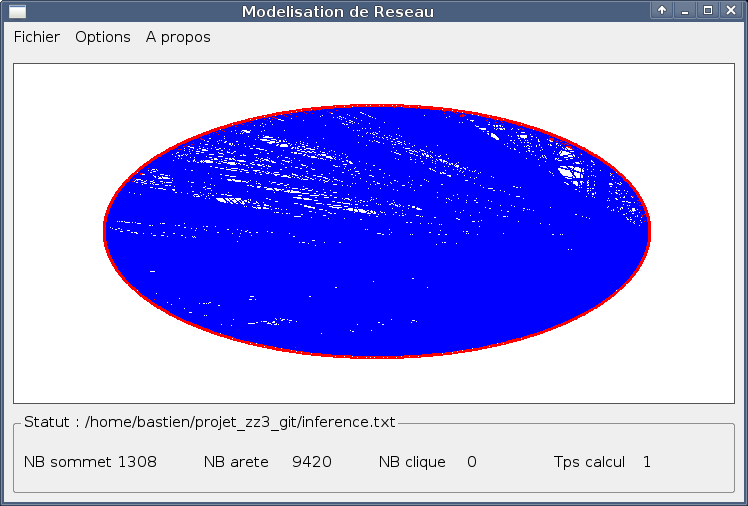
\includegraphics[width=16cm]{./schema/capture_ecran_graph.png}
 }
  \caption{\label{ecran_graph}Ecran principal du programme}
\end{figure}

\subsection{Mise en évidence des caractéristiques d'internet}
%TODO en fonction de ce que l'on a...

\subsection{Bilan}
